This study simulates energy usage in software. The main objective was to simulate a home's energy usage for an entire year in 1-hour increments. In this study, simulations were conducted using data for the entirety of year 2016. Having data for all of 2016 enabled predictions to be used for the aspects of the program that needed them, and then real values to be used for final calculations. It is written in Python and utilizes many Python libraries.

Components of this simulator can be broken up into three distinct areas:

\begin{itemize}
  \item \textbf{Prediction:} mechanisms to enable other components to make informed decisions
  \item \textbf{Decision:} uses predictions to estimate costs of available moves and determine which move is best
  \item \textbf{Outcome:} determines the actual cost of a decision
\end{itemize}

\begin{figure}
 \begin{center}
  \begin{tabular}{cc}
   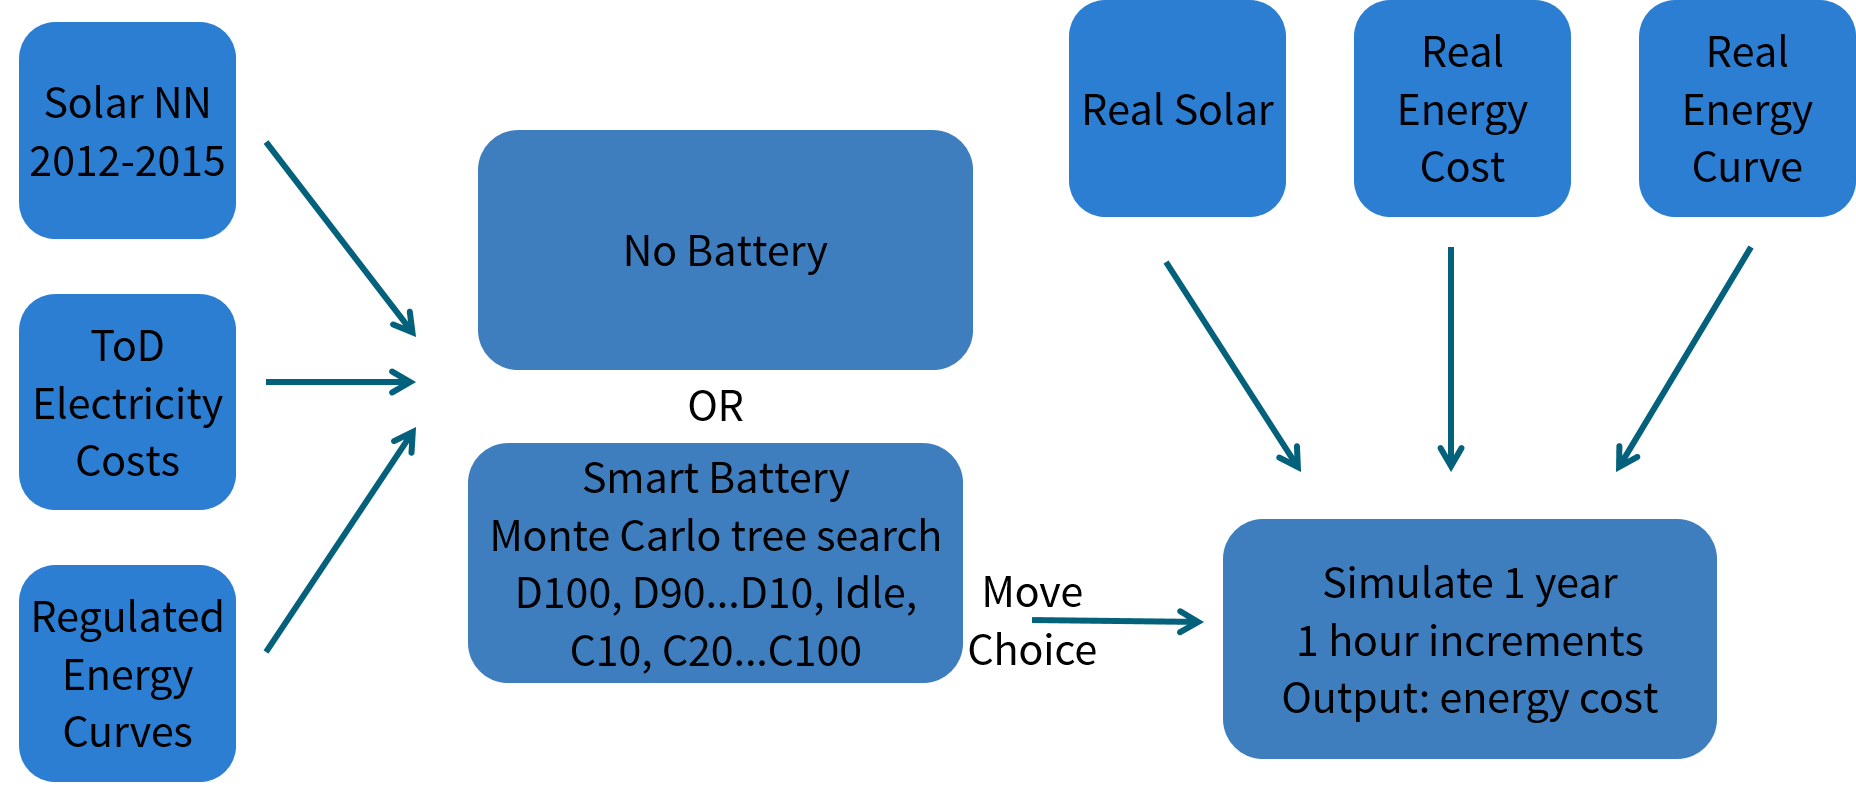
\includegraphics[width=0.50\textwidth]{./figures/image_1.png} \\
   \end{tabular}
   \end{center}
\caption{The layout of the simulation program}
  \vspace{+1mm}
\label{program_layout}
\end{figure}

Figure \ref{program_layout} represents the layout of the simulation program. The bubbles on the left represent \textbf{prediction} components, the boxes in the middle represent the \textbf{decision} components, and the right-side portion represents the \textbf{outcome} components.

\subsection{Prediction: mechanisms to enable other components to make informed decisions}

The simulator allows for several prediction mechanisms.

\begin{itemize}
  \item \textbf{Solar:} Solar prediction is done using a neural network. The actual details of this network are part of a different study. This neural network is trained on information from all of 2012-2015. The inputs for this neural network are time of the day, day of the year, temperature, precipitation, and forecast sky visibility. This information was obtained from several local sources, including Apogee Instruments in Logan Utah, as well as the Logan Utah airport. In getting estimates from the neural network, it was decided to use the actual, measured values of these conditions for 2016 as the predicted values. While this many not be entirely accurate, 24-hour forecasts are accurate enough that it is anticipated the differences will not be drastic. For future studies, some noise could be added to these values to better simulate real conditions.
  \item \textbf{Time-of-day Energy Pricing:} For this paper, time-of-day energy pricing information was obtained from Rocky Mountain power. Rocky Mountain power posts time-of-day pricing that schedules every hour into either off-peak or on-peak pricing. Off-peak pricing yields a discount of \$0.01401 per kWh of energy consumed off-peak, and an additional charge of \$0.04376 per kWh of energy consumed on-peak, per the schdule shown in Figure \ref{tod_pricing} . The base rate was determined \$0.1075 per kWh, taken from an author's monthly energy bill. Thus, given a time of the day, day of the year, and the year, the predictor returns the real cost of energy for that time. The simulator has facilities in place for more robust time-of-day pricing information, such as those proposed for the future updating pricing in 15-minute or other intervals, but these features were not implemented at this time.
  \item \textbf{Home Energy usage:} The home energy predictor is intended to represent two different homes, one a typical home with typical energy-usage habits, and the other a "smart home". A smart home is assumed to contain smart appliances and other enhancements that allow energy usage to be coordinated and scheduled to occur at different times. The goal is that a smart home might have a flatter daily power curve, where electrical loads that might typically occur simultaneously in the evening are intead dispersed more evenly to low-use periods of the day, such as late night and early morning.

  For this paper, two energy curves were obtained from a study conducted by Oracle \cite{fischer_we_2014} where over 800,000 power curves were studied to determine consumer energy usage patterns. It was found that most curves could be lumped into five different categories. The most common was termed the "evening peaker", representing nearly half of all users. The evening peaker does as you might expect and has a peak-load in the evenings that is significantly higher than other loads throughout the day. Another curve, termed the "steady eddy", is nearly flat, with mild increases in usage in the morning and evening. For the purpose of this paper, it was assumed the steady eddy curve is what might be possible with a smart home. Both energy curves are normalized to consume the same total amount of energy over the course of a day. Thus, the curves might not represent a "smart home" in terms of reducing overall energy consumption, but they do allow study of whether shifting loads to off-peak hours is valuable. The actual curves  an be found in Figure \ref{energy_curves}.

  \begin{figure}
   \begin{center}
    \begin{tabular}{cc}
     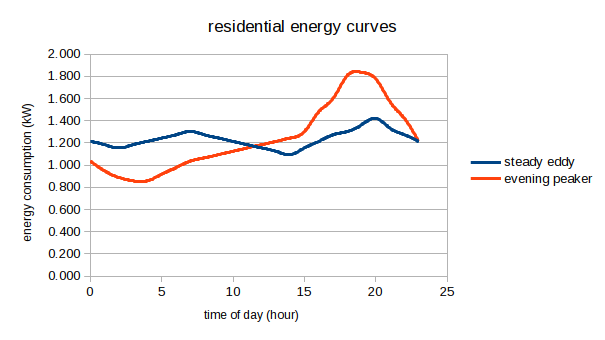
\includegraphics[width=0.50\textwidth]{./figures/energy_curves.png} \\
     \end{tabular}
     \end{center}
  \caption{Energy curves used for this experiment. Both curves represent idential energy usage over 24 hours.}
    \vspace{+1mm}
  \label{energy_curves}
  \end{figure}

  Using the time of day, the home energy usage predictor simply references the power curve of the simulated home to determine power usage for any hour. The simulator is set up to allow for more varied predictions if supplied.
\end{itemize}

\begin{figure}
 \begin{center}
  \begin{tabular}{cc}
   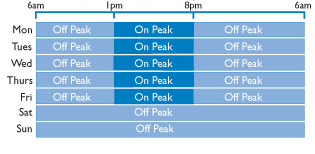
\includegraphics[width=0.50\textwidth]{./figures/utah_tod_pricing.png} \\
   \end{tabular}
   \end{center}
\caption{Time-of-day pricing breakdown for Utah}
  \vspace{+1mm}
\label{tod_pricing}
\end{figure}

\subsection{Decision: uses predictions to estimate costs of available moves and determine which move is best}

The decision component of the simulator has access to all predictors but not the actual values. This was done to represent real conditions as accurately as possible.

The decision process only comes into play when a battery is present. The purpose of the decision process is to look at all the options the battery has at each hour of the day and choose the best option. For this paper, the battery uses the Monte Carlo tree search method. 

Monte Carlo Tree Search involves random sampling of states to completion. It is typically broken down into the following steps \cite{noauthor_monte_2016}:

\begin{enumerate}
  \item \textbf{Selection:} from the starting game state, use some sort of heuristic to choose a next game state to explore
  \item \textbf{Expansion:} from this chosen next game state, randomly choose a further game state to explore
  \item \textbf{Simulation:} randomly choose moves to simulate a game until a win or loss state is encountered
  \item \textbf{Backpropagation:} traverse back to the starting game state, using the simulation results to update corresponding nodes
\end{enumerate}

While there are plenty of papers detailing the use of Monte Carlo tree search for use in perfect information, 2-player games \cite{takeuchi_evaluation_2008} \cite{browne_survey_2012}, there is little research looking at Monte Carlo tree search as a tool in a single player game \cite{schadd_single-player_2012}. However, Monte Carlo tree search seems like a good fit for a battery charging decision algorithm. At every point, there are a contrained number of choices for what a battery can do. The battery has ideas about what might happen in the future, but does not know for sure. In addition, the choices the battery makes now will have an impact on future perfomance. Monte Carlo tree search is a good option that allows a battery to simulate making a decision and then playing out a random simulation to completion. The method includes facilities for determining which pathways to explore. When simulations are complete, the algorithm determines which of all the possible choices puts the battery in the best position in the future.

There were a few details to work out with single player Monte Carlo tree search that are not a problem in typical applications.
\begin{itemize}
    \item Typical Monte Carlo tree search completes a simulation when a game is either won, lost, or drawn. For the simulations in this paper, the simulation will actually complete after a specified number of rounds, such as 24. Each round represents one hour into the future to take into consideration. Once the round limit has been reached, the total cost of all the decisions made to that point is calculated, and that value is used to back propagate through the algorithm.
    \item In a perfect information 2-player game, there is typically a winner and loser. A binary score is thus typically enough for rewarding Monte Carlo tree search simulations. However, in the application in our paper, the reward is instead based on how much electricity a system has to purchase from the energy grid. Thus, the number can be any value starting at 0 (there is also possibility of net metering or earning credits for producing more energy than you consume, which is ignored in this paper). In order for the statistical sampling of the algorithm to work correctly, somehow these unbounded values need to be constrained to something between 0 and 1. Eventually, the equation \(1 - \frac{cost}{cost + 1}\) was settled on. With this equation, the closer a value is to \$0 cost, the closer the reward is to the max value of 1. Likewise, as the cost increases, the reward approaches 0. This equation was adequate for the method to work.
    \item For Monte Carlo tree search to work, there need to be choices of moves to make. "Idle" is always a choice, where the battery chooses to do nothing. However, the battery cannot simply "charge" or "discharge", as there are different rates of both. Thus, it was decided to allow for the battery to charge or discharge at any rate from 10-100\% of the max rate of the battery, in increments of 10\%. This yields 21 possible options for the battery to choose from. The algorithm ensures that options are not available in each round that would overcharge or overdischarge the battery.
\end{itemize}

Once the battery makes a decision on the best action for the next hour, that decision is sent to the outcome portion of the simulator.

\subsection{Outcome: determines the actual cost of a decision}

This final component is fairly basic. The main job of this component is to determine the actual cost of energy at each point in time. If there is no battery present, the system simply looks at how much energy is being consumed by a system, how much energy is entering a system, and how much of that energy had to be purchased from the utility company and at what price. A battery can either be feeding into or pulling from the system, depending on whether it has chosen to charge or discharge for a period of time. The outcome module simply puts all of this together and returns the actual cost of energy for the specific time period in question, and also updates the battery charge state as needed.

Thus, all the parts of the simulator boil down to a few basic inputs of time of day, day of year, and year, and come out as a single number representing cost.